%\documentclass{article}
%\usepackage{graphicx,subfigure}
%\begin{document}

\begin{figure}[!h]
  \centering
  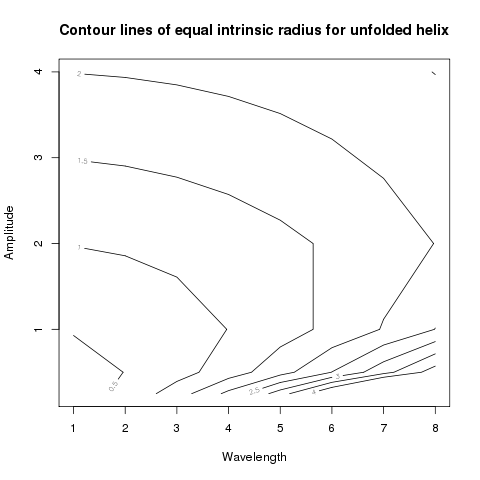
\includegraphics[width=1.0\textwidth]{Rplot002.png}
%   Rplot002.png is original 
  \caption{Contour diagram showing the mathematical relationship between crimp amplitude, crcrimp wavelength, and intrinsic radius of fibre curvature. Countour lines of equal radius of curvature at variuos combinations of amplitude and wavelength are shown to be highly nonlinear}
  \label{fig:nonlin}
\end{figure}

%\end{document}

